\section{Reference-group phase diagnostics}

\begin{frame}{Physical symmetry is relative to a background}
  \bookref{Chapter 6, Section 1}
  A physical domain carries background structure $B$ before a phase is chosen:
  geometry, adjacency, species, interactions, locality, and boundary data.
  \[
    \boxed{G\leq\Aut(B)},
    \qquad
    H_S=\{g\in G:g\cdot S=S\}.
  \]

  For finite index,
  \[
    I_G(S)=\log[G:H_S].
  \]

  \begin{alertblock}{Modeling requirement}
    Arbitrary site permutations and exchanges of distinct chemical species are
    excluded unless they genuinely preserve the background theory.
  \end{alertblock}

  Symmetry-related states have conjugate stabilizers, so $I_G$ is constant on
  every $G$-orbit.
\end{frame}

\begin{frame}{Diagnostics for continuous states and phase limits}
  \bookref{Chapter 6, Sections 2--4}
  \centering
  \begin{tabular}{lll}
    \toprule
    diagnostic & records & caution \\
    \midrule
    \shortstack[l]{finite-window\\rate} &
      \shortstack[l]{thermodynamic scaling\\of symmetry loss} &
      \shortstack[l]{exhaustion and\\boundary dependence} \\
    \shortstack[l]{quotient $G/H$ and\\$\dim(G/H)$} &
      \shortstack[l]{continuous broken\\directions} &
      no statistical weight \\
    $D_{\mathrm{KL}}(\nu\Vert\mu_{G/H})$ &
      \shortstack[l]{concentration relative to\\invariant phase measure} &
      \shortstack[l]{resolution and\\measure dependence} \\
    \bottomrule
  \end{tabular}

  \vspace{0.7em}
  \begin{block}{Discrete baseline}
    $\log[G:H]$ remains exact for finite symmetry reductions, point groups,
    chirality choices, and order--disorder sectors. Continuous symmetry can
    already occur at finite system size.
  \end{block}
\end{frame}

\begin{frame}{Why the diagnostics must remain distinct}
  \bookref{Chapter 6, Sections 2 and 4}
  A broken global $\mathbb Z_2$ symmetry has
  \[
    I_L=\log 2,
    \qquad
    \frac{I_L}{|X_L|}\longrightarrow0.
  \]
  The zero rate does not undo the broken discrete symmetry; it says that the
  orbit choice is subextensive.

  \vspace{0.5em}
  For compact $G$, raw Haar measure of $H$ is positive exactly at finite index.
  Continuous ordering is instead probed by a phase law $\nu$ on $G/H$:
  \[
    I_{\mathrm{meas}}(\nu\mid\mu)
      =D_{\mathrm{KL}}(\nu\Vert\mu)\geq0.
  \]

  \begin{block}{Interpretation}
    Index detects discrete sectors; rate detects scaling; quotient geometry
    detects broken directions; relative entropy detects statistical selection.
  \end{block}
\end{frame}

\begin{frame}{Computed $SO(2)$ orientational transition}
  \bookref{Chapter 6, Section 5}
  \begin{columns}[T,onlytextwidth]
    \begin{column}{0.70\textwidth}
      \centering
      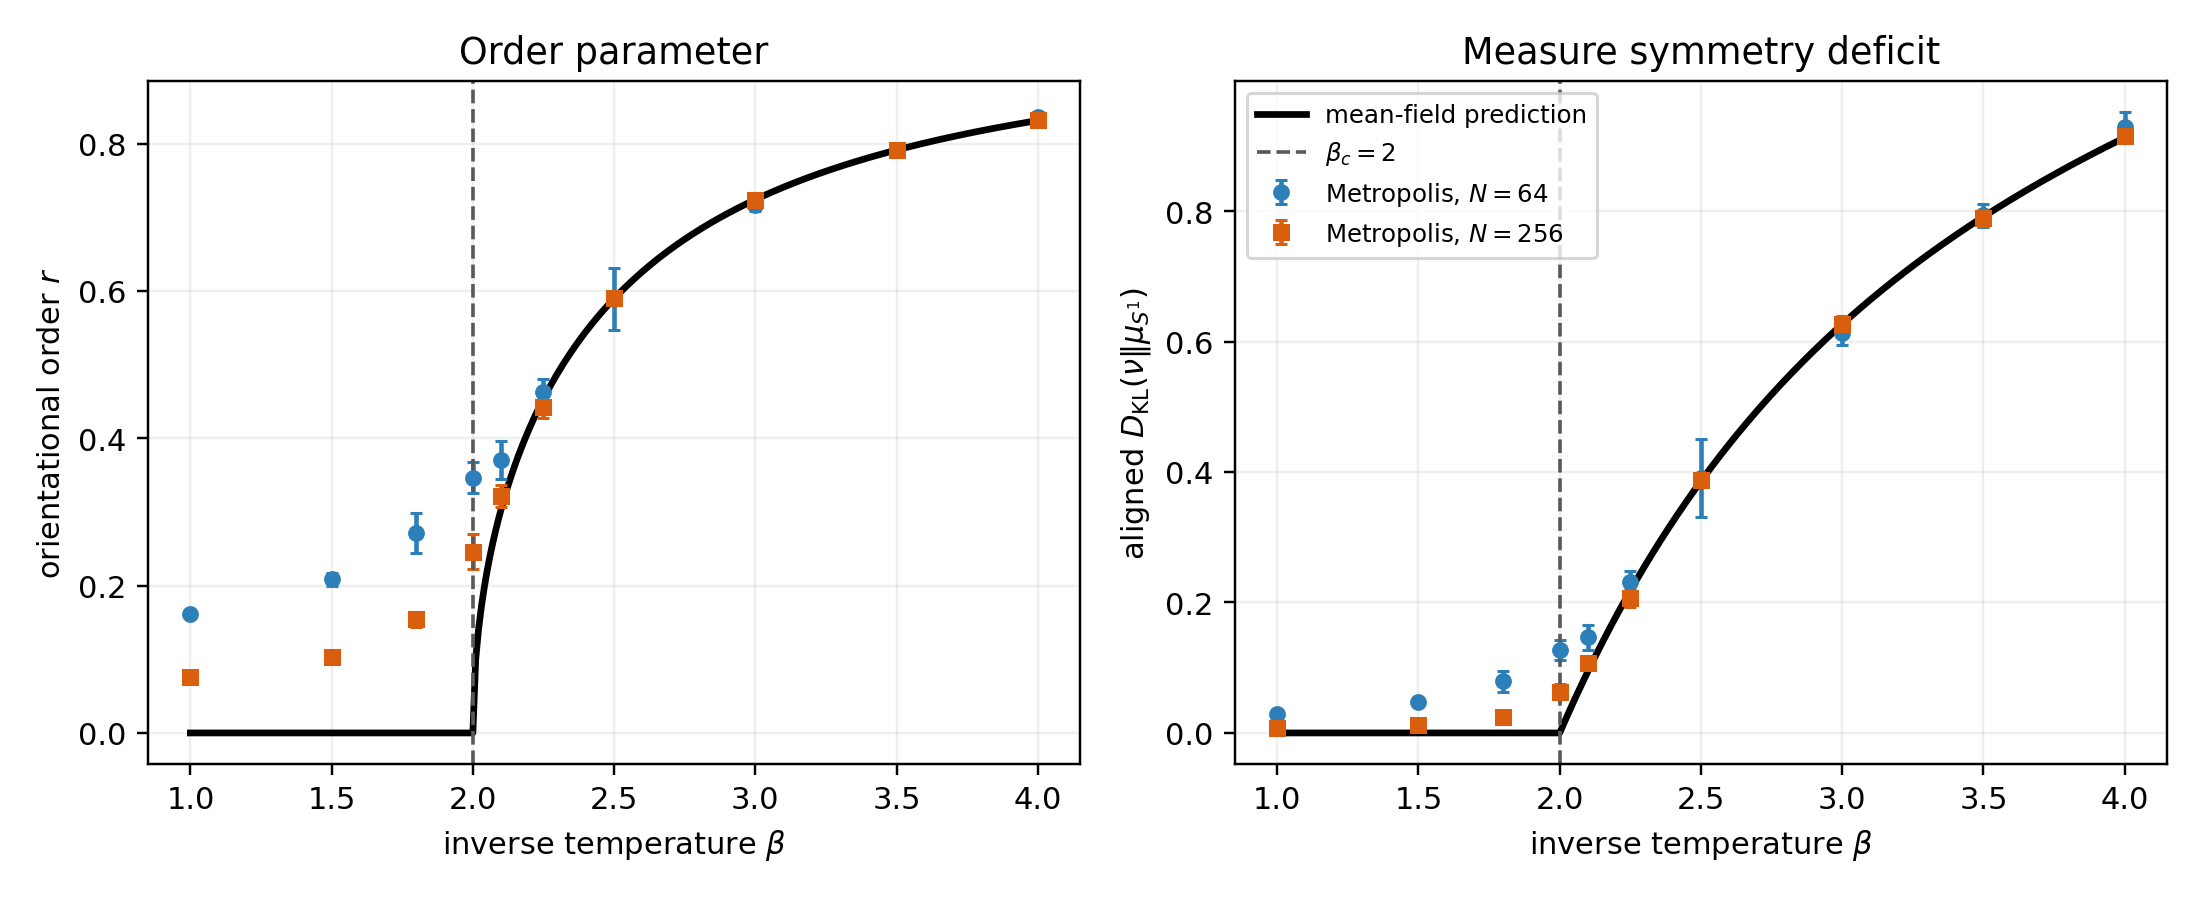
\includegraphics[width=\textwidth]{reference_group_xy_transition.png}
    \end{column}
    \begin{column}{0.28\textwidth}
      \footnotesize
      \[
        r=\frac{I_1(\beta Jr)}{I_0(\beta Jr)},
        \qquad \beta_cJ=2.
      \]
      For the selected phase,
      \[
        D_{\mathrm{KL}}
        =\beta Jr^2-\log I_0(\beta Jr).
      \]
      At $\beta=3$, $N=256$:
      \begin{align*}
        r_{\rm sim}&=0.723995,\\
        r_{\rm pred}&=0.724159.
      \end{align*}
      Alignment selects a branch and creates the visible finite-$N$ bias below
      the transition.
    \end{column}
  \end{columns}
\end{frame}

\begin{frame}{Interacting Bose ensembles add a spectral diagnostic}
  \bookref{Chapter 6, Section 7}
  \small
  For the one-particle reduced density operator,
  \[
    \gamma^{(1)}=N\operatorname{Tr}_{2,\ldots,N}\Gamma,
    \qquad
    c_{\mathrm{BEC}}
      =\liminf\frac{\lambda_{\max}(\gamma^{(1)})}{N}.
  \]
  The cited OpenAI preprint reports (not independently proved here) $c_{\mathrm{BEC}}>0$ for the exact
  canonical Gibbs state at a fixed positive density and a positive temperature
  independent of volume \cite{openai2026bec}.

  \begin{columns}[T]
    \column{0.48\textwidth}
      \begin{block}{Shared geometry}
        A separately phase-selected one-component state has
        \[
          G/H=U(1)/\{1\}\cong S^1,
        \]
        with soft phase twists in its effective Goldstone sector.
      \end{block}
    \column{0.48\textwidth}
      \begin{alertblock}{Distinct invariants}
        $c_{\mathrm{BEC}}$ is not $i_G$, and a macroscopic eigenvalue is not the
        block proxy $(p-q)^2$. A fixed-$N$ canonical state remains
        $U(1)$-invariant even when it has ODLRO.
      \end{alertblock}
  \end{columns}
\end{frame}

\begin{frame}{One quotient language, two separate theorems}
  \bookref{Chapter 6, Section 7}
  \small
  \begin{center}
    \begin{tabular}{lll}
      \toprule
      OpenAI result & order statement & main mechanism \\
      \midrule
      \shortstack[l]{interacting hard-sphere\\Bose gas} &
      \shortstack[l]{macroscopic constant-\\orbital occupation} &
      \shortstack[l]{thermal paths and\\density-matrix overlap} \\
      \shortstack[l]{quantum Heisenberg\\ferromagnet} &
      \shortstack[l]{selected zero-field\\KMS magnetization} &
      \shortstack[l]{exchange paths and\\boundary pinning} \\
      \bottomrule
    \end{tabular}
  \end{center}

  \vspace{0.6em}
  The branch manifolds fit the same reference-group framework:
  \[
    U(1)/\{1\}\cong S^1,
    \qquad
    SO(3)/SO(2)\cong S^2.
  \]
  \begin{block}{Scope}
    Shared quotient geometry does not make ODLRO, magnetization, a deficit
    rate, and a block-density invariant mathematically identical
    \cite{openai2026ferromagnet}.
  \end{block}
\end{frame}
